\iffalse
This file is protected by Copyright. Please refer to the COPYRIGHT file
distributed with this source distribution.

This file is part of OpenCPI <http://www.opencpi.org>

OpenCPI is free software: you can redistribute it and/or modify it under the
terms of the GNU Lesser General Public License as published by the Free Software
Foundation, either version 3 of the License, or (at your option) any later
version.

OpenCPI is distributed in the hope that it will be useful, but WITHOUT ANY
WARRANTY; without even the implied warranty of MERCHANTABILITY or FITNESS FOR A
PARTICULAR PURPOSE. See the GNU Lesser General Public License for more details.

You should have received a copy of the GNU Lesser General Public License along
with this program. If not, see <http://www.gnu.org/licenses/>.
\fi

%----------------------------------------------------------------------------------------
% Update the docTitle and docVersion per document
%----------------------------------------------------------------------------------------
\def\docTitle{OpenCPI\\ FSK App Guide}
\def\docVersion{1.5}
%----------------------------------------------------------------------------------------
\def\snippetpath{../../../../../doc/av/tex/snippets}
% Usage:
% \def\snippetpath{../../../../../doc/av/tex/snippets/}
% % Usage:
% \def\snippetpath{../../../../../doc/av/tex/snippets/}
% % Usage:
% \def\snippetpath{../../../../../doc/av/tex/snippets/}
% \input{\snippetpath/includes}
% From then on, you can use "input" With no paths to get to "snippets"
% You also get all "major" snippets not part of the global LaTeX_Header
% NOTE: If not using the global LaTeX_Header, you need to
% \usepackage{ifthen} to use the \githubio macro

\hyphenation{ANGRY-VIPER} % Tell it where to hyphenate
\hyphenation{Cent-OS} % Tell it where to hyphenate
\hyphenation{install-ation} % Tell it where to hyphenate

\newcommand{\todo}[1]{\textcolor{red}{TODO: #1}\PackageWarning{TODO:}{#1}} % To do notes
\newcommand{\code}[1]{\texttt{#1}} % For inline code snippet or command line
\newcommand{\sref}[1]{Section~\ref{#1}} % To quickly reference a section

% To quickly reference a versioned PDF on gitlab.io
\def\ocpiversion{develop}

% This gives a link to gitlab.io document. By default, it puts the filename.
% You can optionally change the link, e.g.
% \githubio{FPGA\_Vendor\_Tools\_Installation\_Guide.pdf} vs.
% \githubio[\textit{FPGA Vendor Tools Installation Guide}]{FPGA\_Vendor\_Tools\_Installation\_Guide.pdf}
% or if you want the raw ugly URL to come out, \githubioURL{FPGA_Vendor_Tools_Installation_Guide.pdf}
\newcommand{\githubio}[2][]{% The default is for FIRST param!
\href{http://opencpi.gitlab.io/releases/\ocpiversion/docs/#2}{\ifthenelse{\equal{#1}{}}{\texttt{#2}}{#1}}}
\newcommand{\gitlabcom}[2][]{% The default is for FIRST param!
\href{http://gitlab.com/opencpi/#2}{\ifthenelse{\equal{#1}{}}{\texttt{#2}}{#1}}}
\newcommand{\githubioURL}[1]{\url{http://opencpi.gitlab.io/releases/\ocpiversion/docs/#1}}
% Lastly, if you want a SINGLE leading path stripped, e.g. assets/X.pdf => X.pdf:
\newcommand{\githubioFlat}[1]{%
\StrBehind{#1}{/}[\den]%
\href{http://opencpi.gitlab.io/releases/\ocpiversion/docs/#1}{\texttt{\den}}%
}

% Fix import paths
\makeatletter
\def\input@path{{\snippetpath/}}
\makeatother

% From then on, you can use "input" With no paths to get to "snippets"
% You also get all "major" snippets not part of the global LaTeX_Header
% NOTE: If not using the global LaTeX_Header, you need to
% \usepackage{ifthen} to use the \githubio macro

\hyphenation{ANGRY-VIPER} % Tell it where to hyphenate
\hyphenation{Cent-OS} % Tell it where to hyphenate
\hyphenation{install-ation} % Tell it where to hyphenate

\newcommand{\todo}[1]{\textcolor{red}{TODO: #1}\PackageWarning{TODO:}{#1}} % To do notes
\newcommand{\code}[1]{\texttt{#1}} % For inline code snippet or command line
\newcommand{\sref}[1]{Section~\ref{#1}} % To quickly reference a section

% To quickly reference a versioned PDF on gitlab.io
\def\ocpiversion{develop}

% This gives a link to gitlab.io document. By default, it puts the filename.
% You can optionally change the link, e.g.
% \githubio{FPGA\_Vendor\_Tools\_Installation\_Guide.pdf} vs.
% \githubio[\textit{FPGA Vendor Tools Installation Guide}]{FPGA\_Vendor\_Tools\_Installation\_Guide.pdf}
% or if you want the raw ugly URL to come out, \githubioURL{FPGA_Vendor_Tools_Installation_Guide.pdf}
\newcommand{\githubio}[2][]{% The default is for FIRST param!
\href{http://opencpi.gitlab.io/releases/\ocpiversion/docs/#2}{\ifthenelse{\equal{#1}{}}{\texttt{#2}}{#1}}}
\newcommand{\gitlabcom}[2][]{% The default is for FIRST param!
\href{http://gitlab.com/opencpi/#2}{\ifthenelse{\equal{#1}{}}{\texttt{#2}}{#1}}}
\newcommand{\githubioURL}[1]{\url{http://opencpi.gitlab.io/releases/\ocpiversion/docs/#1}}
% Lastly, if you want a SINGLE leading path stripped, e.g. assets/X.pdf => X.pdf:
\newcommand{\githubioFlat}[1]{%
\StrBehind{#1}{/}[\den]%
\href{http://opencpi.gitlab.io/releases/\ocpiversion/docs/#1}{\texttt{\den}}%
}

% Fix import paths
\makeatletter
\def\input@path{{\snippetpath/}}
\makeatother

% From then on, you can use "input" With no paths to get to "snippets"
% You also get all "major" snippets not part of the global LaTeX_Header
% NOTE: If not using the global LaTeX_Header, you need to
% \usepackage{ifthen} to use the \githubio macro

\hyphenation{ANGRY-VIPER} % Tell it where to hyphenate
\hyphenation{Cent-OS} % Tell it where to hyphenate
\hyphenation{install-ation} % Tell it where to hyphenate

\newcommand{\todo}[1]{\textcolor{red}{TODO: #1}\PackageWarning{TODO:}{#1}} % To do notes
\newcommand{\code}[1]{\texttt{#1}} % For inline code snippet or command line
\newcommand{\sref}[1]{Section~\ref{#1}} % To quickly reference a section

% To quickly reference a versioned PDF on gitlab.io
\def\ocpiversion{develop}

% This gives a link to gitlab.io document. By default, it puts the filename.
% You can optionally change the link, e.g.
% \githubio{FPGA\_Vendor\_Tools\_Installation\_Guide.pdf} vs.
% \githubio[\textit{FPGA Vendor Tools Installation Guide}]{FPGA\_Vendor\_Tools\_Installation\_Guide.pdf}
% or if you want the raw ugly URL to come out, \githubioURL{FPGA_Vendor_Tools_Installation_Guide.pdf}
\newcommand{\githubio}[2][]{% The default is for FIRST param!
\href{http://opencpi.gitlab.io/releases/\ocpiversion/docs/#2}{\ifthenelse{\equal{#1}{}}{\texttt{#2}}{#1}}}
\newcommand{\gitlabcom}[2][]{% The default is for FIRST param!
\href{http://gitlab.com/opencpi/#2}{\ifthenelse{\equal{#1}{}}{\texttt{#2}}{#1}}}
\newcommand{\githubioURL}[1]{\url{http://opencpi.gitlab.io/releases/\ocpiversion/docs/#1}}
% Lastly, if you want a SINGLE leading path stripped, e.g. assets/X.pdf => X.pdf:
\newcommand{\githubioFlat}[1]{%
\StrBehind{#1}{/}[\den]%
\href{http://opencpi.gitlab.io/releases/\ocpiversion/docs/#1}{\texttt{\den}}%
}

% Fix import paths
\makeatletter
\def\input@path{{\snippetpath/}}
\makeatother

\iffalse
This file is protected by Copyright. Please refer to the COPYRIGHT file
distributed with this source distribution.

This file is part of OpenCPI <http://www.opencpi.org>

OpenCPI is free software: you can redistribute it and/or modify it under the
terms of the GNU Lesser General Public License as published by the Free Software
Foundation, either version 3 of the License, or (at your option) any later
version.

OpenCPI is distributed in the hope that it will be useful, but WITHOUT ANY
WARRANTY; without even the implied warranty of MERCHANTABILITY or FITNESS FOR A
PARTICULAR PURPOSE. See the GNU Lesser General Public License for more details.

You should have received a copy of the GNU Lesser General Public License along
with this program. If not, see <http://www.gnu.org/licenses/>.
\fi

% Sets OpenCPI Version used throughout all the docs. This is updated by
% scripts/update-release.sh when a release is being made and must not
% be changed manually.
\def\ocpiversion{v2.2.0}

\documentclass{article}
\author{}  % Force author to be blank
\date{OpenCPI Release:\ \ \ocpiversion}  % Force date to be blank and override date with version
\title{OpenCPI\\\docTitle}  % docTitle must be defined before including this file
%----------------------------------------------------------------------------------------
% Paper size, orientation and margins
%----------------------------------------------------------------------------------------
\usepackage{geometry}
\geometry{
  letterpaper,  % paper type
  portrait,     % text direction
  left=.75in,   % left margin
  top=.75in,    % top margin
  right=.75in,  % right margin
  bottom=.75in  % bottom margin
}
%----------------------------------------------------------------------------------------
% Header/Footer
%----------------------------------------------------------------------------------------
\usepackage{fancyhdr} \pagestyle{fancy}  % required for fancy headers
\renewcommand{\headrulewidth}{0.5pt}
\renewcommand{\footrulewidth}{0.5pt}
\lhead{\small{\docTitle}}
\rhead{\small{OpenCPI}}
%----------------------------------------------------------------------------------------
% Various packages
%----------------------------------------------------------------------------------------
\usepackage{amsmath}
\usepackage[page,toc]{appendix}  % for appendix stuff
\usepackage{enumitem}
\usepackage{graphicx}   % for including pictures by file
\usepackage{hyperref}   % for linking urls and lists
\usepackage{listings}   % for coding language styles
\usepackage{pdflscape}  % for landscape view
\usepackage{pifont}     % for sideways table
\usepackage{ragged2e}   % for justify
\usepackage{rotating}   % for sideways table
\usepackage{scrextend}
\usepackage{setspace}
\usepackage{subfig}
\usepackage{textcomp}
\usepackage[dvipsnames,usenames]{xcolor}  % for color names see https://en.wikibooks.org/wiki/LaTeX/Colors
\usepackage{xstring}
\uchyph=0  % Never hyphenate acronyms like RCC
\renewcommand\_{\textunderscore\allowbreak}  % Allow words to break/newline on underscores
%----------------------------------------------------------------------------------------
% Table packages
%----------------------------------------------------------------------------------------
\usepackage[tableposition=top]{caption}
\usepackage{float}
\floatstyle{plaintop}
\usepackage{longtable}  % for long possibly multi-page tables
\usepackage{multicol}   % for more advanced table layout
\usepackage{multirow}   % for more advanced table layout
\usepackage{tabularx}   % c=center,l=left,r=right,X=fill
% These define tabularx columns "C" and "R" to match "X" but center/right aligned
\newcolumntype{C}{>{\centering\arraybackslash}X}
\newcolumntype{M}[1]{>{\centering\arraybackslash}m{#1}}
\newcolumntype{P}[1]{>{\centering\arraybackslash}p{#1}}
\newcolumntype{R}{>{\raggedleft\arraybackslash}X}
%----------------------------------------------------------------------------------------
% Block Diagram / FSM Drawings
%----------------------------------------------------------------------------------------
\usepackage{tikz}
\usetikzlibrary{arrows,decorations.markings,fit,positioning,shapes}
\usetikzlibrary{automata}  % used for the fsm
\usetikzlibrary{calc}      % for duplicating clients
\usepgfmodule{oo}          % to define a client box
%----------------------------------------------------------------------------------------
% Colors Used
%----------------------------------------------------------------------------------------
\usepackage{colortbl}
\definecolor{blue}{rgb}{.7,.8,.9}
\definecolor{ceruleanblue}{rgb}{0.16, 0.32, 0.75}
\definecolor{cyan}{rgb}{0.0,0.6,0.6}
\definecolor{darkgreen}{rgb}{0,0.6,0}
\definecolor{deepmagenta}{rgb}{0.8, 0.0, 0.8}
\definecolor{maroon}{rgb}{0.5,0,0}
%----------------------------------------------------------------------------------------
% Define where to hyphenate
%----------------------------------------------------------------------------------------
\hyphenation{Cent-OS}
\hyphenation{install-ation}
%----------------------------------------------------------------------------------------
% Define Commands & Rename Commands
%----------------------------------------------------------------------------------------
\newcommand{\code}[1]{\texttt{#1}}  % For inline code snippet or command line
\newcommand{\sref}[1]{Section~\ref{#1}}  % To quickly reference a section
\newcommand{\todo}[1]{\textcolor{red}{TODO: #1}\PackageWarning{TODO:}{#1}}  % To do notes
\renewcommand{\contentsname}{Table of Contents}
\renewcommand{\listfigurename}{List of Figures}
\renewcommand{\listtablename}{List of Tables}

% This gives a link to gitlab.io document. By default, it outputs the filename.
% You can optionally change the link, e.g.
% \githubio{FPGA\_Vendor\_Tools\_Installation\_Guide.pdf} vs.
% \githubio[\textit{FPGA Vendor Tools Installation Guide}]{FPGA\_Vendor\_Tools\_Installation\_Guide.pdf}
% or if you want the raw ugly URL to come out, \githubioURL{FPGA_Vendor_Tools_Installation_Guide.pdf}
\newcommand{\githubio}[2][]{% The default is for FIRST param!
\href{http://opencpi.gitlab.io/releases/\ocpiversion/docs/#2}{\ifthenelse{\equal{#1}{}}{\texttt{#2}}{#1}}}
\newcommand{\gitlabcom}[2][]{% The default is for FIRST param!
\href{http://gitlab.com/opencpi/#2}{\ifthenelse{\equal{#1}{}}{\texttt{#2}}{#1}}}
\newcommand{\githubioURL}[1]{\url{http://opencpi.gitlab.io/releases/\ocpiversion/docs/#1}}
% Lastly, if you want a SINGLE leading path stripped, e.g. assets/X.pdf => X.pdf:
\newcommand{\githubioFlat}[1]{%
\StrBehind{#1}{/}[\den]%
\href{http://opencpi.gitlab.io/releases/\ocpiversion/docs/#1}{\texttt{\den}}%
}
%----------------------------------------------------------------------------------------
% VHDL Coding Language Style
% modified from: http://latex-community.org/forum/viewtopic.php?f=44&t=22076
%----------------------------------------------------------------------------------------
\lstdefinelanguage{VHDL}
{
  basicstyle=\ttfamily\footnotesize,
  columns=fullflexible,keepspaces,  % https://tex.stackexchange.com/a/46695/87531
  keywordstyle=\color{ceruleanblue},
  commentstyle=\color{darkgreen},
  morekeywords={
    library, use, all, entity, is, port, in, out, end, architecture, of,
    begin, and, signal, when, if, else, process, end,
  },
  morecomment=[l]--
}
%----------------------------------------------------------------------------------------
% XML Coding Language Style
% modified from http://tex.stackexchange.com/questions/10255/xml-syntax-highlighting
%----------------------------------------------------------------------------------------
\lstdefinelanguage{XML}
{
  basicstyle=\ttfamily\footnotesize,
  columns=fullflexible,keepspaces,
  morestring=[s]{"}{"},
  morecomment=[s]{!--}{--},
  commentstyle=\color{darkgreen},
  moredelim=[s][\color{black}]{>}{<},
  moredelim=[s][\color{cyan}]{\ }{=},
  stringstyle=\color{maroon},
  identifierstyle=\color{ceruleanblue}
}
%----------------------------------------------------------------------------------------
% DIFF Coding Language Style
% modified from http://tex.stackexchange.com/questions/50176/highlighting-a-diff-file
%----------------------------------------------------------------------------------------
\lstdefinelanguage{diff}
{
  basicstyle=\ttfamily\footnotesize,
  columns=fullflexible,keepspaces,
  breaklines=true,                            % wrap text
  morecomment=[f][\color{ceruleanblue}]{@@},  % group identifier
  morecomment=[f][\color{red}]-,              % deleted lines
  morecomment=[f][\color{darkgreen}]+,        % added lines
  morecomment=[f][\color{deepmagenta}]{---},  % Diff header lines (must appear after +,-)
  morecomment=[f][\color{deepmagenta}]{+++},
}
%----------------------------------------------------------------------------------------
% Python Coding Language Style
%----------------------------------------------------------------------------------------
\lstdefinelanguage{python}
{
  basicstyle=\ttfamily\footnotesize,
  columns=fullflexible,keepspaces,
  keywordstyle=\color{ceruleanblue},
  commentstyle=\color{darkgreen},
  stringstyle=\color{orange},
  morekeywords={
    print, if, sys, len, from, import, as, open,close, def, main, for, else,
    write, read, range,
  },
  comment=[l]{\#}
}
%----------------------------------------------------------------------------------------
% Fontsize Notes in order from smallest to largest
%----------------------------------------------------------------------------------------
%    \tiny
%    \scriptsize
%    \footnotesize
%    \small
%    \normalsize
%    \large
%    \Large
%    \LARGE
%    \huge
%    \Huge

\date{Version \docVersion} % Force date to be blank and override date with version
\title{\docTitle}
\lhead{FSK App Guide}
%----------------------------------------------------------------------------------------
%\usepackage[T1]{fontenc} % http://tex.stackexchange.com/a/181119
\usepackage{graphicx}
\graphicspath{ {figures/} }
\usepackage{textcomp}

\begin{document}
\maketitle
%\thispagestyle{fancy}
\newpage
	\begin{center}
	\textit{\textbf{Revision History}}
		\begin{table}[H]
		\label{table:revisions} % Add "[H]" to force placement of table
			\begin{tabularx}{\textwidth}{|c|X|l|}
			\hline
			\rowcolor{blue}
			\textbf{Revision} & \textbf{Description of Change} & \textbf{Date} \\
		    \hline
		    v1.1 & Initial Release & 3/2017 \\
		    \hline
		    v1.2 & Updated for OpenCPI Release 1.2 & 8/2017 \\
			\hline
			v1.3 & Updated for OpenCPI Release 1.3 & 1/2018 \\
			\hline
			v1.3.1 & Updated for OpenCPI Release 1.3.1, including FMCOMMS2/3 support & 3/2018 \\
			\hline
			v1.4 & Updated recommendations for configuring OCPI\_LIBRARY\_PATH & 9/2018 \\
			\hline
			v1.5 & Deprecated Zipper; Moved to Appendix & 3/2019 \\
			\hline
			\end{tabularx}
		\end{table}
	\end{center}

\newpage
\tableofcontents
\pagebreak
\section{Document Scope}
This document describes the OpenCPI FSK demo application. It includes a description of the application, instructions to setup the hardware, build of bitstreams, and execution of the application itself on various platforms.

\section{Supported Hardware Setups}
This app is supported on the following hardware configurations:
\begin{itemize}
  \item Zedboard/FMCOMMS2
  \item Zedboard/FMCOMMS3
  \item x86/ML605/FMCOMMS2 in FMC LPC slot
  \item x86/ML605/FMCOMMS3 in FMC LPC slot
  \item Matchstiq-Z1
\end{itemize}

\section{Description}
The FSK App may be run in one of five available modes. The modes are \textit{filerw}, \textit{rx}, \textit{tx}, \textit{txrx}, and \textit{bbloopback}. The \textit{filerw} mode uses file\_read and file\_write workers to process the input using only application workers (platform agnostic) in a purely digital fashion. A block diagram of the FSK App \textit{filerw} mode can be seen in Figure \ref{fig:filerw_mode_block_diagram}.
	\begin{figure}[H]
	 	\centering
		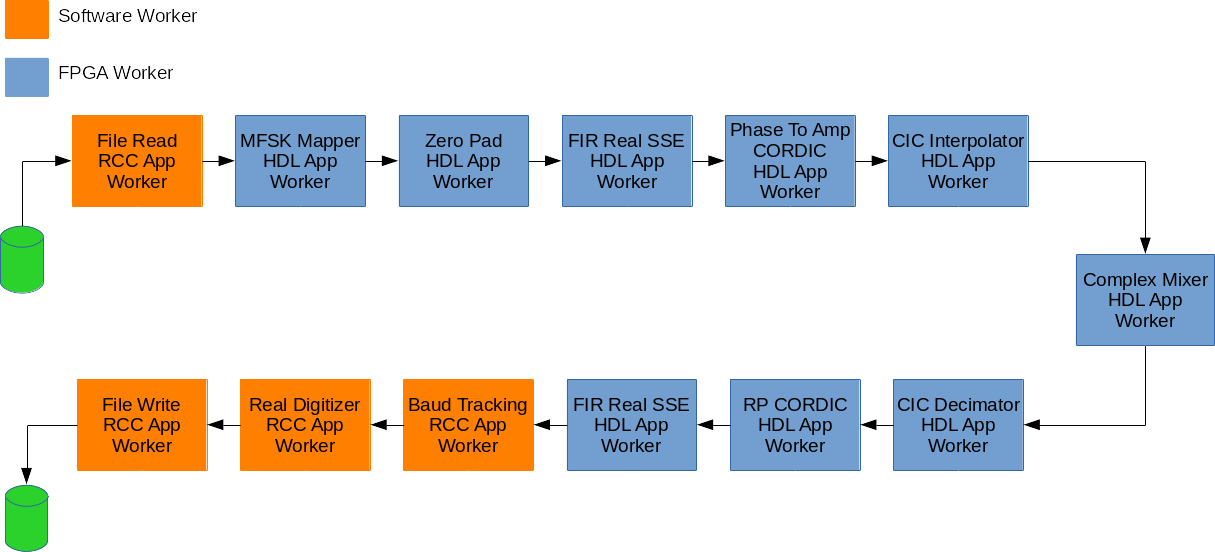
\includegraphics[scale=.55]{filerw_mode_block_diagram}
		\caption{FSK App \textit{filerw} mode Block Diagram}
		\label{fig:filerw_mode_block_diagram}
	\end{figure}

\newpage
\noindent The \textit{rx} mode inputs IQ data from the Lime ADC and processes the FSK signal down to bits that are written to file. A block diagram of the FSK App \textit{rx} mode can be seen in Figure \ref{fig:rx_mode_block_diagram}.\par\medskip
	\begin{figure}[H]
	 	\centering
		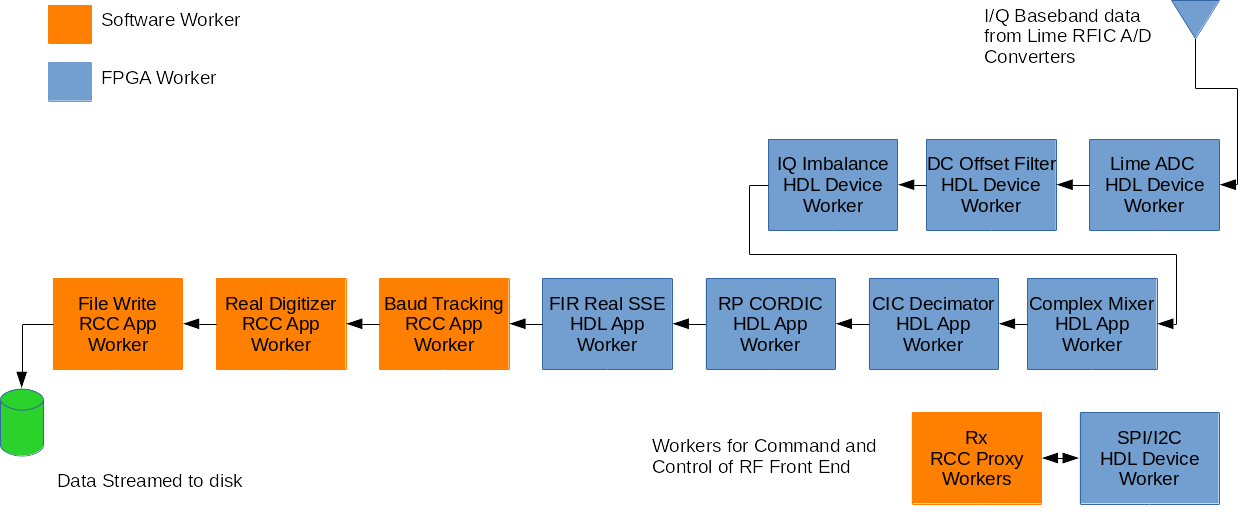
\includegraphics[scale=.55]{rx_mode_block_diagram}
		\caption{FSK App \textit{rx} mode Block Diagram}
		\label{fig:rx_mode_block_diagram}
	\end{figure}

\noindent The \textit{tx} mode inputs a file from disk, modulates the input as a FSK signal, and transmits the input via the Lime DAC. A block diagram of the FSK App \textit{tx} mode can be seen in Figure \ref{fig:tx_mode_block_diagram}.
	\begin{figure}[H]
	 	\centering
		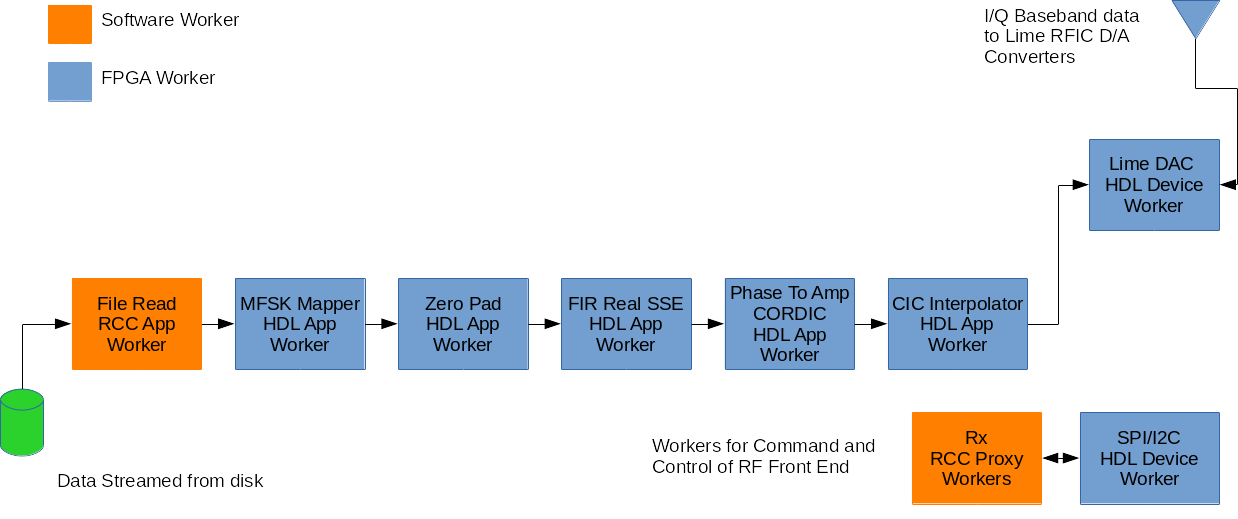
\includegraphics[scale=.55]{tx_mode_block_diagram}
		\caption{FSK App \textit{tx} mode Block Diagram}
		\label{fig:tx_mode_block_diagram}
	\end{figure}

\noindent The \textit{txrx} mode is the full transceiver mode of the application which combines the functionality of Figures \ref{fig:rx_mode_block_diagram} and \ref{fig:tx_mode_block_diagram} into a single application. This mode transmits input file data as the radio RF TX output and inputs RF RX radio input that is written to file. The \textit{bbloopback} mode utilizes the same HDL assembly and application XML as the \textit{txrx} mode but utilizes a built-in test mode of the Lime transceiver to loopback analog data at baseband.\par\medskip

\noindent The \textit{tx}, \textit{txrx}, and \textit{bbloopback} modes for the Matchstiq-Z1 contain the matchstiq\_z1\_gp\_out device worker which can control the three GPIO pins present on the Matchstiq-Z1. The application XMLs give an example of how to use the device worker.\par\medskip
\subsection{Application Specifications}
\subsubsection{Baud Rate}
The baud rate for the application is based on the following properties:
	\begin{itemize}
		\item ADC/DAC Sample Rate (S)
		\item CIC Decimation/Interpolation Factor (R)
		\item Number of zeros inserted between symbols (Z)
	\end{itemize}
It can be computed using the following equation:
	      \begin{equation} \label{eq:cic_gain}
	      	Baud\ Rate = S\ /\ R\ /\ (Z +1)
	      \end{equation}
Using the default settings for the Ettus E310 platform, the resulting baud rate is approximately 6.4K baud.
	      \begin{equation} \label{eq:cic_gain}
	      	Baud\ Rate = S\ /\ R\ /\ (Z+1) = 4e6 \ /\ 16\ /\ (38+1) \ =\ 6410
	      \end{equation}
\subsubsection{Frequency Deviation}
The frequency deviation for the application is based on the following characteristics of the application:
	\begin{itemize}
		\item Pulse shaping FIR output amplitude (fir\_output)
		\item Width of data (DATA\_WIDTH)
		\item CIC Decimation/Interpolation Factor (R)
		\item ADC/DAC Sample Rate (S)
	\end{itemize}
After the bits of the input file are mapped to symbols, zeros are inserted in between symbols. After zero padding, the output is pulse shaped by a root raised cosine FIR filter. The taps of the filter are configurable and should be based on the expected baud rate of the application. See \texttt{applications/FSK/scripts/gen\_rrcos\_taps.py} for more information. Using the default tap values, the output of the filter ranges from approximately +3300 to -3300. These output values from the FIR determine the min and max frequencies produced by the phase\_to\_amp\_cordic according to the following equation.
	\begin{equation} \label{eq:output_freq}
		cordic\_freq = \frac{fir\_output}{2^{DATA\_WIDTH}} = \frac{+/-3300}{2^{16}} = +/- 0.0504\ cycles\ per\ sample
	\end{equation}
The output of the CORDIC is upsampled by a interpolating CIC filter. The output data of the CIC is passed to the DAC, which has a configurable sample rate. The resulting output frequency of the DAC is defined by:
	\begin{equation} \label{eq:output_freq}
		output\_freq = cordic\_freq\ /\ R\ *\ S
	\end{equation}
Using the default settings for the Ettus E310 platform, the resulting frequency deviation is approximately 12588 Hz with mark and space frequencies at 2400012588 Hz and 2399987411 Hz.
	\begin{equation} \label{eq:output_freq}
		output\_freq = cordic\_freq\ /\ R\ *\ S = 0.717\ /\ 16\ *\ 4e6 \ =\ 12588\ Hz
	\end{equation}

\newpage
\section{Building the Application}
\subsection{Dependencies}
\noindent The tables below breakdown the workers used within the various platforms and modes of the FSK App. Appendix~\ref{app:Worker_Parameters} shows the exact worker configurations used in the HDL assemblies. See the individual component data sheets for more information and build instructions. Similarly, the HDL platform worker and configurations for the intended radio must be compiled prior to building the various FSK bitstreams.
\subsection{FSK Mode Configurations}
\subsubsection{Common to all Hardware}
	\begin{tabular}{|c|c|c|c|c|c|}
	\hline
	\rowcolor{blue}
	Application XML & filerw & rx & tx & txrx & bbloopback \\
	\hline
	app\_fsk\_filerw (dependency only, no build required) & x & • & • & • & • \\
	\rowcolor{blue}
	HDL Assemblies & filerw & rx & tx & txrx & bbloopback \\
	\hline
	fsk\_filerw & x & • & • & • & • \\
	\hline
	dc\_offset\_iq\_imbalance\_mixer\_cic\_dec\_rp\_cordic\_fir\_real & • & x & • & • & • \\
	\hline
	mfsk2\_zp16\_fir\_real\_phase\_to\_amp\_cordic\_cic\_int & • & • & x & • & • \\
	\hline
	fsk\_modem & • & • & • & x & x \\
	\hline
	\rowcolor{blue}
	RX Path Workers & filerw & rx & tx & txrx & bbloopback \\
	\hline
	dc\_offset\_filter.hdl & • & x & • & x & x \\
	\hline
	iq\_imbalance\_fixer.hdl & • & x & • & x & x \\
	\hline
	complex\_mixer.hdl & x & x & • & x & x \\
	\hline
	cic\_dec.hdl & x & x & • & x & x \\
	\hline
	rp\_cordic.hdl & x & x & • & x & x \\
	\hline
	fir\_real\_sse.hdl & x & x & • & x & x \\
	\hline
	baudTracking.rcc & x & x & • & x & x \\
	\hline
	real\_digitizer.rcc & x & x & • & x & x \\
	\hline
	file\_write.rcc & x & x & • & x & x \\
	\hline
	\rowcolor{blue}
	TX Path Workers & filerw & rx & tx & txrx & bbloopback \\
	\hline
	file\_read.rcc & x & • & x & x & x \\
	\hline
	mfsk\_mapper.hdl & x & • & x & x & x \\
	\hline
	zero\_pad.hdl & x & • & x & x & x \\
	\hline
	fir\_real\_sse.hdl & x & • & x & x & x \\
	\hline
	phase\_to\_amp\_cordic.hdl & x & • & x & x & x \\
	\hline
	cic\_int.hdl & x & • & x & x & x \\
	\hline
	\end{tabular}

\subsubsection{Additional Dependencies for FMCOMMS2}
	\begin{tabular}{|c|c|c|c|c|c|}
	\hline
	\rowcolor{blue}
	Application XML & filerw & rx & tx & txrx & bbloopback \\
	\hline
	app\_fsk\_rx\_fmcomms2 (dependency only, no build required) & • & x & • & • & • \\
	\hline
	app\_fsk\_tx\_fmcomms2 (dependency only, no build required) & • & • & x & • & • \\
	\hline
	app\_fsk\_txrx\_fmcomms2 (dependency only, no build required) & • & •  & • & x & • \\
	\hline
	\rowcolor{blue}
	RX or TX Path Workers & filerw & rx & tx & txrx & bbloopback \\
	\hline
	ad9361\_data\_sub.hdl & • & x & x & x & • \\
	\rowcolor{blue}
	RX Path Workers & filerw & rx & tx & txrx & bbloopback \\
	\hline
	ad9361\_adc.hdl & • & x & • & x & • \\
	\hline
	ad9361\_adc\_sub.hdl & • & x & • & x & • \\
	\hline
	\rowcolor{blue}
	TX Path Workers & filerw & rx & tx & txrx & bbloopback \\
	\hline
	ad9361\_dac.hdl & • & • & x & x & • \\
	\hline
	ad9361\_dac\_sub.hdl & • & • & x & x & • \\
	\rowcolor{blue}
	Endpoint Proxies & filerw & rx & tx & txrx & bbloopback \\
	\hline
	fmcomms\_2\_3\_rx.rcc & • & x & • & x & • \\
	\hline
	fmcomms\_2\_3\_tx.rcc & • & • & x & x & • \\
	\hline
	\rowcolor{blue}
	SPI Command and Control & filerw & rx & tx & txrx & bbloopback \\
	\hline
	ad9361\_config.hdl & • & x & x & x & • \\
	\hline
	ad9361\_config\_proxy.rcc & • & x & x & x & •  \\
	\hline
	ad9361\_spi.hdl & • & x & x & x &   \\
	\hline
	\rowcolor{blue}
	I2C Command and Control & filerw & rx & tx & txrx & bbloopback \\
	\hline
	fmcomms\_2\_3\_i2c.hdl & • & x & x & x &   \\
	\hline
	\end{tabular}

\subsubsection{Additional Dependencies for FMCOMMS3}
	\begin{tabular}{|c|c|c|c|c|c|}
	\hline
	\rowcolor{blue}
	Application XML & filerw & rx & tx & txrx & bbloopback \\
	\hline
	app\_fsk\_rx\_fmcomms3 (dependency only, no build required) & • & x & • & • & • \\
	\hline
	app\_fsk\_tx\_fmcomms3 (dependency only, no build required) & • & • & x & • & • \\
	\hline
	app\_fsk\_txrx\_fmcomms3 (dependency only, no build required) & • & •  & • & x & • \\
	\hline
	\rowcolor{blue}
	RX or TX Path Workers & filerw & rx & tx & txrx & bbloopback \\
	\hline
	ad9361\_data\_sub.hdl & • & x & x & x & • \\
	\rowcolor{blue}
	RX Path Workers & filerw & rx & tx & txrx & bbloopback \\
	\hline
	ad9361\_adc.hdl & • & x & • & x & • \\
	\hline
	ad9361\_adc\_sub.hdl & • & x & • & x & • \\
	\hline
	\rowcolor{blue}
	TX Path Workers & filerw & rx & tx & txrx & bbloopback \\
	\hline
	ad9361\_dac.hdl & • & • & x & x & • \\
	\hline
	ad9361\_dac\_sub.hdl & • & • & x & x & • \\
	\rowcolor{blue}
	Endpoint Proxies & filerw & rx & tx & txrx & bbloopback \\
	\hline
	fmcomms\_2\_3\_rx.rcc & • & x & • & x & • \\
	\hline
	fmcomms\_2\_3\_tx.rcc & • & • & x & x & • \\
	\hline
	\rowcolor{blue}
	SPI Command and Control & filerw & rx & tx & txrx & bbloopback \\
	\hline
	ad9361\_config.hdl & • & x & x & x & • \\
	\hline
	ad9361\_config\_proxy.rcc & • & x & x & x & •  \\
	\hline
	ad9361\_spi.hdl & • & x & x & x &   \\
	\hline
	\rowcolor{blue}
	I2C Command and Control & filerw & rx & tx & txrx & bbloopback \\
	\hline
	fmcomms\_2\_3\_i2c.hdl & • & x & x & x &   \\
	\hline
	\end{tabular}





\subsubsection{Additional Dependencies for Matchstiq-Z1}
	\begin{tabular}{|c|c|c|c|c|c|}
	\hline
	\rowcolor{blue}
	Application XML & filerw & rx & tx & txrx & bbloopback \\
	\hline
	app\_fsk\_rx\_matchstiq\_z1 (dependency only, no build required) & • & x & • & • & • \\
	\hline
	app\_fsk\_tx\_matchstiq\_z1 (dependency only, no build required) & • & • & x & • & • \\
	\hline
	app\_fsk\_txrx\_matchstiq\_z1 (dependency only, no build required) & • & • & • & x & x \\
	\hline
	\rowcolor{blue}
	RX Path Workers & filerw & rx & tx & txrx & bbloopback \\
	\hline
	lime\_adc.hdl & • & x & • & x & x \\
	\hline
	\rowcolor{blue}
	TX Path Workers & filerw & rx & tx & txrx & bbloopback \\
	\hline
	lime\_dac.hdl & • & • & x & x & x \\
	\hline
	\rowcolor{blue}
	Endpoint Proxies & filerw & rx & tx & txrx & bbloopback \\
	\hline
	matchstiq\_z1\_rx.rcc & • & x & • & x & x \\
	\hline
	matchstiq\_z1\_tx.rcc & • & • & x & x & x \\
	\hline
	\rowcolor{blue}
	SPI Command and Control & filerw & rx & tx & txrx & bbloopback \\
	\hline
	lime\_rx\_proxy.rcc & • & x & • & x & x \\
	\hline
	lime\_rx.hdl & • & x & • & x & x \\
	\hline
	lime\_tx\_proxy.rcc & • & • & x & x & x \\
	\hline
	lime\_tx.hdl & • & • & x & x & x \\
	\hline
	lime\_spi.hdl & • & x & x & x & x \\
	\hline
	\rowcolor{blue}
	I2C Command and Control & filerw & rx & tx & txrx & bbloopback \\
	\hline
	si5338\_proxy.rcc & • & x & x & x & x \\
	\hline
	si5338.hdl & • & x & x & x & x \\
	\hline
	matchstiq\_z1\_avr\_proxy.rcc & • & x & x & x & x \\
	\hline
	matchstiq\_z1\_avr.hdl & • & x & x & x & x \\
	\hline
	tmp100\_proxy.rcc & • & x & x & x & x \\
	\hline
	tmp100.hdl & • & x & x & x & x \\
	\hline
	matchstiq\_z1\_pca9535\_proxy.rcc & • & x & x & x & x \\
	\hline
	pca9535.hdl & • & x & x & x & x \\
	\hline
	matchstiq\_z1\_i2c.hdl & • & x & x & x & x \\
	\hline
	\end{tabular}


	\newpage
\begin{landscape}
\subsection{Performance and Resource Utilization}
\subsubsection{filerw}
\input{../../../hdl/assemblies/fsk_filerw/utilization.inc}
\subsubsection{tx}
\input{../../../hdl/assemblies/mfsk2_zp16_fir_real_phase_to_amp_cordic_cic_int/utilization.inc}
\subsubsection{rx}
\input{../../../hdl/assemblies/dc_offset_iq_imbalance_mixer_cic_dec_rp_cordic_fir_real/utilization.inc}
\subsubsection{txrx/bbloopback}
\input{../../../hdl/assemblies/fsk_modem/utilization.inc}
\end{landscape}
\subsection{Executable}
The software portion of the application consists of a C++ program written using the OpenCPI C++ API as well as RCC proxy workers for command and control functionality. The program references the appropriate application XML file for the requested hardware and mode. The app XML files contain all of the property settings for the components in each application, except for the configuration of the endpoint proxy(ies). These endpoint proxy-related settings are passed via command-line prompted values to the appropriate endpoint proxy workers.\\
To build for the host platform (which is the case if ML605 or Stratix IV platform is intended to be used), run the following commands from the FSK directory:\par\medskip
\texttt{ ocpidev build}\par\medskip
\noindent To build for the Zedboard or Matchstiq-Z1 (which run the xilinx13\_3 PetaLinux operating system), run the following command from the FSK directory:\par\medskip
\texttt{ ocpidev build --rcc-platform xilinx13\_3 }\par\medskip

\section{Testing the Application}
\subsection{Baud Synchronization}
The input filename for the application is idata/Os.jpeg. It is modified from an original JPEG image (see Figure \ref{fig:os_pic}) with data prepended to it for baud synchronization purposes (240 bytes of an alternating 1-0 pattern followed by 2 bytes are the value 0xFACE). In the receive data stream, real\_digitizer.rcc worker makes symbol/bit decisions and only sends out bits that occur after the first detected 0xFACE bit pattern (b1111101011001110). The image is also padded with 40 bytes of zeros. This padding ensures that all image data is pushed through the signal processing chain.
\subsection{Sample test setup}
The test setup varies per mode of operation. The base test setup includes a hardware platform of choice and appropriate power and USB cables (Matchstiq-Z1 uses the USB cable to access the terminal via a program such as \textit{screen} or over a USB-over-Ethernet connection; Stratix IV and ML605 require a USB cable for JTAG loading). All other test modes expand upon this base configuration, and may or may not include additional RF cabling or external equipment.\par\medskip
\noindent The \textit{filerw} mode requires only the base test setup since no transceiver operations are actuated (data passes to and from the FPGA in a ``loopback'' fashion). Upon application execution, the expected result is written to odata/out\_app\_fsk\_filerw.bin, which is a transmitted copy of the input file idata/Os.jpeg, without the prepended synchronizing pattern.\par\medskip
\noindent The \textit{bbloopback} mode is similar to the \textit{filerw} mode, but data goes beyond the FPGA through the radio's built-in analog baseband loopback, and back into the FPGA. Because the data never reaches the TX/RX connectors, no external RF cabling is required. The expected result is a transmitted copy of the idata/Os.jpeg file as the output odata/out\_app\_fsk\_bbloopback.bin, without the prepended synchronizing pattern. Since this test is executed for a duration, rather than total image recognition, it is not uncommon that the output file will be larger than the actual size of the input image.\par\medskip
\noindent The next mode is the \textit{rx} mode, which requires the base test setup with an RX antenna, as well as another transmitter (such as another platform running the \textit{tx} mode) in order to broadcast a known FSK signal. Optionally, a spectrum analyzer may be connected to the transmitter to visually verify that the signal being fed into the radio's RX input is an FSK signal at the correct RF frequency and bandwidth. The output is written to the file odata/out\_app\_fsk\_rx.bin, without the prepended synchronizing pattern. Since this test is executed for a duration, rather than total image recognition, it is not uncommon that the output file will be larger than the actual size of the input image.\par\medskip
\noindent The next mode is the \textit{tx} mode, which requires the base test setup with a TX antenna, as well as some hardware to verify the transmission, such as a spectrum analyzer or an additional radio running in \textit{rx} mode. In this mode the input file idata/Os.jpeg is transmitted out of the RF TX output of the radio.\par\medskip
\noindent The final mode is the \textit{txrx} mode. This mode requires a base test setup with either a SMA loopback cable connecting the TX output of the radio to the RX input of the radio, or separate RX/TX antennas if RF usage is desired. An RF splitter can also be used to optionally connect a spectrum analyzer to the RF signal for visual verification. The default values for RF gain assume that an RF splitter is being used. The output is written to the file odata/out\_app\_fsk\_txrx.bin, without the prepended synchronizing pattern. Since this test is executed for a duration, rather than total image recognition, it is not uncommon that the output file will be larger than the actual size of the input image.
\par\medskip
\subsection{make show}
In order to test the application using the various modes mentioned above, \texttt{make show} can be run from the \texttt{applications/FSK} directory. This provides instructions (for Zynq-Based Platforms) for setting \texttt{OCPI\_LIBRARY\_PATH} on the hardware platform and then running the application. Finally, it explains how to verify the output data on the development computer. The following sections provide further insight into these instructions.
\subsection{Artifacts}
Before running the application, the location of the required deployable artifacts must be specified in the \texttt{OCPI\_LIBRARY\_PATH} environment variable. Separate artifacts are needed for each RCC worker, and one artifact for the required FPGA image. Furthermore, artifacts differ depending on which mode the application is to be run in. Appendix~\ref{app:Artifacts} includes a list of the artifacts required for each platform and mode.
\subsection{Arguments to executable}
There is only one required initial argument to the FSK App executable, which defines the mode of execution. There is an optional initial argument to the FSK App executable that defines whether or not to run in debug mode. The app prompts the user at runtime for additional values, which vary depending upon the selected mode of operation. Running the application without any arguments prints the usage instructions. The non-initial optional arguments prompt the user to override the default value(s), and primarily configure the RF front end of the given platform using one or more endpoint proxies.\par\medskip
\noindent The arguments to the executable are summarized in the following table:\\
\begin{tabular}{|l|l|l|}
\hline
\rowcolor{blue}
Argument & Mode & Description \\
\hline
mode & n/a & filerw, rx, tx, txrx, bbloopback\\
\hline
debug\_mode & optional - `d' or blank & enables initial and final dump of all properties\\
\hline
\end{tabular}\par\bigskip
\noindent The prompts performed by the executable are summarized in the following table:\\
\begin{tabular}{|l|l|p{6.5cm}|}
\hline
\rowcolor{blue}
Argument & Mode & Description \\
\hline
RF frontend (ML605 and zed only) & rx, txrx & zipper, FMCOMMS2, or FMCOMMS3\\
\hline
runtime & filerw, rx, tx, txrx, bbloopback & run time of application in seconds\\
\hline
rx\_sample\_rate & rx, txrx, bbloopback & RX RF sample rate in Msps\\
\hline
rx\_rf\_center\_freq & rx, txrx, bbloopback & RX RF tuning frequency in MHz\\
\hline
rx\_rf\_bw & rx, txrx, bbloopback & RX RF bandwidth in MHz\\
\hline
rx\_rf\_gain & rx, txrx, bbloopback & RX RF gain in dB\\
\hline
rx\_bb\_bw & rx, txrx, bbloopback & RX baseband bandwidth in MHz\\
\hline
rx\_bb\_gain & rx, txrx, bbloopback & RX baseband gain in dB\\
\hline
rx\_if\_center\_freq & rx, txrx, bbloopback & RX IF tuning frequency in MHz. 0 disables IF tuning\\
\hline
tx\_sample\_rate & tx, txrx, bbloopback & TX RF sample rate in Msps\\
\hline
tx\_rf\_center\_freq & tx, txrx, bbloopback & TX RF tuning frequency in MHz\\
\hline
tx\_rf\_gain & tx, txrx, bbloopback & TX RF gain in dB\\
\hline
tx\_bb\_bw & tx, txrx, bbloopback & TX baseband bandwidth in MHz\\
\hline
tx\_bb\_gain & tx, txrx, bbloopback & TX baseband gain in dB\\
\hline
\end{tabular}\par\medskip
\pagebreak
\noindent Example arguments for the \textbf{FMCOMMS2} card using the txrx mode with an SMA loopback cable between FMCOMMS2 SMA ports RX1A and TX1A:\\
\begin{tabular}{|l|l|}
\hline
\rowcolor{blue}
Parameter 	&        Value  	\\
\hline
RF frontend 	&        FMCOMMS2             	\\
\hline
Runtime (s) 	&        20 	        \\
\hline
RX SMA channel 	&        RX1A              	\\
\hline
TX SMA channel 	&        TX1A           	\\
\hline
rx\_sample\_rate 	&4 	                \\
\hline
rx\_rf\_center\_freq 	&2400 (default)  	\\
\hline
rx\_rf\_bw 	&        -1 (default)   \\
\hline
rx\_rf\_gain 	&        24       	\\
\hline
rx\_bb\_bw 	&        4 	        \\
\hline
rx\_bb\_gain 	&        -1 (default) 	\\
\hline
rx\_if\_center\_freq 	&0              	\\
\hline
tx\_sample\_rate 	&4              	\\
\hline
tx\_rf\_center\_freq 	&2400 (default)\\
\hline
tx\_rf\_bw 	&        -1 (default)   \\
\hline
tx\_rf\_gain 	&        -34 	        \\
\hline
tx\_bb\_bw 	&        4        	\\
\hline
tx\_bb\_gain    &       -1 (default) \\
\hline
\end{tabular}\par\medskip

% \pagebreak
\noindent Example arguments for the \textbf{FMCOMMS3} card using the txrx mode with an SMA loopback cable between FMCOMMS3 SMA ports RX1A and TX1A:\\
\begin{tabular}{|l|l|}
\hline
\rowcolor{blue}
Parameter 	&        Value  	\\
\hline
RF frontend 	&        FMCOMMS3             	\\
\hline
Runtime (s) 	&        20 	        \\
\hline
RX SMA channel 	&        RX1A              	\\
\hline
TX SMA channel 	&        TX1A           	\\
\hline
rx\_sample\_rate 	&4 	                \\
\hline
rx\_rf\_center\_freq 	&2400 (default)  	\\
\hline
rx\_rf\_bw 	&        -1 (default)   \\
\hline
rx\_rf\_gain 	&        24       	\\
\hline
rx\_bb\_bw 	&        4 	        \\
\hline
rx\_bb\_gain 	&        -1 (default) 	\\
\hline
rx\_if\_center\_freq 	&0              	\\
\hline
tx\_sample\_rate 	&4              	\\
\hline
tx\_rf\_center\_freq 	&2400 (default)\\
\hline
tx\_rf\_bw 	&        -1 (default)   \\
\hline
tx\_rf\_gain 	&        -34 	        \\
\hline
tx\_bb\_bw 	&        4        	\\
\hline
tx\_bb\_gain    &       -1 (default) \\
\hline
\end{tabular}\par\medskip

\pagebreak
\subsection{Library Path Requirements}
\noindent Prior to running the application, the environment variable OCPI\_LIBRARY\_PATH must be configure, such that, all of the FSK application's run-time artifacts can be located. OpenCPI conveniently provides access to a project's run-time artifacts at the top-level of each project in a directory called artifacts. Reference the OpenCPI Application Development Guide for more about OCPI\_LIBRARY\_PATH. \par\medskip
\noindent Note that the Stratix IV GX230 and ML605 hardware setups require the intended slot-specific bitstream's file location to be first in OCPI\_LIBRARY\_PATH. This is necessary because ocpirun's aritifact compatibility test does not currently differentiate between slot-connected device workers for multiple bitstreams that contain the same device worker, in the scenario where what differentiates the bitstreams is the device worker's slot connectivity. \par\medskip

\noindent The following are recommendations for configuring the OCPI\_LIBRARY\_PATH based on the mode of FSK, platform, the use of a daughter card and specific slot that card is installed. For all recommendations:
\begin{itemize}
  \item All paths are relative to the applications/FSK/ directory.\\
  \item It is assumed (for PCI/host platforms) that the \code{core} and \code{assets} projects are named as such and exist in the same parent directory.\\
\end{itemize}

\noindent\textbf{Recommended Library Path for Matchstiq-Z1 or Zedboard}\\

\noindent
For these platforms, follow the instructions contained in the FSK application's Makefile. They can be viewed by opening the Makefile in an editor, or by executing ``\code{make show}'' from within the assets/applications/FSK/.\\

\noindent\textbf{Recommended Library Path \textit{filerw} mode for all host/PCI platforms}\\
\noindent
\verb|OCPI_LIBRARY_PATH=../../core/artifacts:../../artifacts| \\

\noindent\textbf{Recommended Library Path for ML605/FMCOMMS2/3-HPC}\\

\noindent
\noindent\textbf{\textit{Not Supported}}\\

\noindent\textbf{Recommended Library Path for ML605/FMCOMMS2/3-LPC}\\

\noindent
\verb|OCPI_LIBRARY_PATH=../../core/artifacts:../../artifacts| \\
\par\medskip

\pagebreak

\subsection{Expected results}
\noindent In the case of the \textit{filerw}, \textit{rx}, \textit{txrx}, and \textit{bbloopback} modes, assuming transmission of the idata/Os.jpeg input file, the expected result is a transmitted copy of the JPEG file. A Linux program such as Eye of GNOME (eog) may be used to display the JPEG file. The file is shown in Figure \ref{fig:os_pic}.\par\medskip
\noindent In the case of the \textit{tx} mode, verification is obtained by viewing the RF spectrum on a spectrum analyzer. An example of the transmitted spectrum may be seen in Figure \ref{fig:tx_spec_an}.\par\medskip
	\begin{figure}[ht]
	 	\centering
	 	\begin{minipage}{.325\textwidth}
			\centering\includegraphics[width=1.0\linewidth]{Os}
			\caption{FSK input file}
			\label{fig:os_pic}
		\end{minipage}
	 	\begin{minipage}{.45\textwidth}
			\centering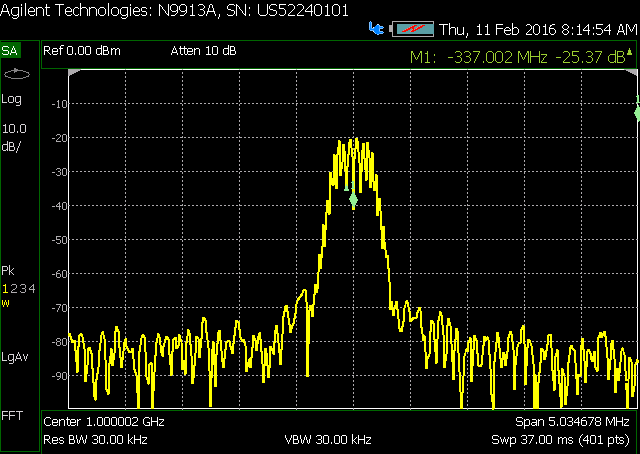
\includegraphics[width=1.0\linewidth]{tx_spec_an}
			\caption{Output of FSK App RF transmit}
			\label{fig:tx_spec_an}
		\end{minipage}
	\end{figure}
% \pagebreak
\subsection{Known Issues}
\noindent
\begin{itemize}
  \item  % AV-4043
    The demodulation algorithm currently suffers from limited carrier
    recovery ability which can cause the output image to be corrupted or
    non-existent
    when using the \textit{rx} or \textit{txrx} mode.
    If using an SMA loopback for txrx mode
    on an RF transceiver where the RX and TX data stream's LOs are sourced by
    the same clock, carrier recovery is not
    expected to be an issue.

\end{itemize}
\begin{appendices}
\section{Worker Parameters}
\label{app:Worker_Parameters}
\begin{minipage}[t]{.5\textwidth}
	\textbf{Common to all hardware}
	\begin{itemize}
		\item dc\_offset\_filter.hdl
			\subitem DATA\_WIDTH\_p = 16
			\subitem PEAK\_MONITOR\_p = true
		\item iq\_imbalance\_fixer.hdl
			\subitem DATA\_WIDTH\_p = 16
			\subitem ACC\_PREC\_p = 38
			\subitem PEAK\_MONITOR\_p = true
		\item complex\_mixer.hdl
			\subitem CHIPSCOPE\_p = false
			\subitem NCO\_DATA\_WIDTH\_p = 12
			\subitem INPUT\_DATA\_WIDTH\_p = 12
			\subitem CORDIC\_STAGES\_p = 16
			\subitem PEAK\_MONITOR\_p = true
		\item cic\_dec.hdl
			\subitem N = 3
			\subitem M = 1
			\subitem R = 16
			\subitem DIN\_WIDTH = 16
			\subitem ACC\_WIDTH = 28
			\subitem DOUT\_WIDTH = 16
		\item rp\_cordic.hdl
			\subitem DATA\_WIDTH = 16
			\subitem DATA\_EXT = 6
			\subitem STAGES = 16
		\item fir\_real\_sse.hdl (rx\_fir\_real)
			\subitem NUM\_TAPS\_p = 64
			\subitem DATA\_WIDTH\_p = 16
			\subitem COEFF\_WIDTH\_p = 16
		\item mfsk\_mapper.hdl
			\subitem M\_p = 2
		\item zero\_pad.hdl
			\subitem DWIDTH\_p = 16
	\end{itemize}
\end{minipage}
\begin{minipage}[t]{.5\textwidth}
	\textbf{ML605 (with FMCOMMS2/3 card in FMC HPC slot)}
	\begin{itemize}
		\item fmcomms\_2\_3\_i2c.hdl
			\subitem CP\_CLK\_FREQ\_p = 125e6
			\subitem FMC\_GA1 = 0
			\subitem FMC\_GA0 = 0
		\item ad9361\_spi.hdl
			\subitem CP\_CLK\_FREQ\_HZ\_p = 125e6
		\item ad9361\_data\_sub.hdl
			\subitem LVDS\_p = true
			\subitem DATA\_CLK\_Delay = 2
			\subitem RX\_Data\_Delay = 0
			\subitem FB\_CLK\_Delay = 7
			\subitem TX\_Data\_Delay = 0
	\end{itemize}
	\textbf{ML605 (with FMCOMMS2/3 card in FMC LPC slot)}
	\begin{itemize}
		\item fmcomms\_2\_3\_i2c.hdl
			\subitem CP\_CLK\_FREQ\_p = 125e6
			\subitem FMC\_GA1 = 1
			\subitem FMC\_GA0 = 0
		\item ad9361\_spi.hdl
			\subitem CP\_CLK\_FREQ\_HZ\_p = 125e6
		\item ad9361\_data\_sub.hdl
			\subitem LVDS\_p = true
			\subitem DATA\_CLK\_Delay = 2
			\subitem RX\_Data\_Delay = 0
			\subitem FB\_CLK\_Delay = 7
			\subitem TX\_Data\_Delay = 0
	\end{itemize}
\end{minipage}

\begin{minipage}[t]{.5\textwidth}
	\textbf{Zedboard FMCOMMS2/3 configurations)}
	\begin{itemize}
		\item fmcomms\_2\_3\_i2c.hdl
			\subitem CP\_CLK\_FREQ\_p = 100e6
			\subitem FMC\_GA1 = 0
			\subitem FMC\_GA0 = 0
		\item ad9361\_spi.hdl
			\subitem CP\_CLK\_FREQ\_HZ\_p = 100e6
		\item ad9361\_data\_sub.hdl
			\subitem LVDS\_p = true
			\subitem DATA\_CLK\_Delay = 2
			\subitem RX\_Data\_Delay = 0
			\subitem FB\_CLK\_Delay = 7
			\subitem TX\_Data\_Delay = 0
	\end{itemize}
\end{minipage}
	\begin{minipage}[t]{.5\textwidth}
		\textbf{Matchstiq-Z1 configurations}
	\begin{itemize}
		\item lime\_adc.hdl
			\subitem DRIVE\_CLK\_p = false
			\subitem USE\_CLK\_IN\_p = false
			\subitem USE\_CTL\_CLK\_p = false
			\subitem USE\_CLK\_OUT\_p = true
		\item si5338.hdl
			\subitem CLKIN\_PRESENT\_p = true
			\subitem CLKIN\_FREQ\_p = 3.072e7
			\subitem XTAL\_PRESENT\_p = false
			\subitem XTAL\_FREQ\_p = 0
			\subitem OUTPUTS\_PRESENT\_p = true, false
			\subitem INTR\_CONNECTED\_p = false
		\item matchstiq\_z1\_i2c.hdl
			\subitem NUSERS\_p = 5
			\subitem SLAVE\_ADDRESS\_p = \\0x45, 0x71, 0x48, 0x21, 0x20
			\subitem CLK\_CNT\_p = 199
	\end{itemize}
		\textbf{Zipper-related platforms (Zedboard, Stratix IV, ML605)}
	\begin{itemize}
		\item lime\_adc.hdl
			\subitem DRIVE\_CLK\_p = false
			\subitem USE\_CLK\_IN\_p = true
			\subitem USE\_CTL\_CLK\_p = false
			\subitem USE\_CLK\_OUT\_p = false
		\item si5351.hdl
			\subitem CLKIN\_PRESENT = true
			\subitem CLKIN\_FREQ = 3.072e7
			\subitem XTAL\_PRESENT = false
			\subitem XTAL\_FREQ = 0
			\subitem VC\_PRESENT = false
			\subitem OUTPUTS\_PRESENT = 0,0,1,1,1,1,0,0
			\subitem OEB\_MODE = low
			\subitem INTR\_CONNECTED = false
		\item zipper\_i2c.hdl
			\subitem NUSERS\_p = 2
	\end{itemize}
	\end{minipage}
	\pagebreak
\section{Artifacts}
\label{app:Artifacts}
\subsection{Zedboard/FMCOMMS2/3}
	\noindent\textbf{filerw (FMCOMMS2/3 not required)}
	\begin{itemize}
	\begin{minipage}[t]{.5\textwidth}
	\item fsk\_filerw\_zed\_base.bitz
	\item target-xilinx13\_3/file\_read.so
	\item target-xilinx13\_3/Baudtracking\_simple.so
	\end{minipage}
	\begin{minipage}[t]{.5\textwidth}
	\item target-xilinx13\_3/real\_digitizer.so
	\item target-xilinx13\_3/file\_write.so
	\end{minipage}
	\end{itemize}

	\noindent\textbf{rx}
	\begin{itemize}
  \item dc\_offset\_iq\_imbalance\_mixer\_cic\_dec\_timestamper\_zed\_cfg\_1rx\_0\\
tx\_fmcomms\_2\_3\_lpc\_lvds\_cnt\_1rx\_0tx\_thruasm\_fmcomms\_2\_3\_lpc\_LVDS\_zed.bitz \\
	\begin{minipage}[t]{.5\textwidth}
	\item target-xilinx13\_3/Baudtracking\_simple.so
	\item target-xilinx13\_3/real\_digitizer.so
	\item target-xilinx13\_3/file\_write.so
	\end{minipage}
	\begin{minipage}[t]{.5\textwidth}
	\item target-xilinx13\_3/ad9361\_config\_proxy.so
	\item target-xilinx13\_3/fmcomms\_2\_3\_rx.so
	\end{minipage}
	\end{itemize}

	\noindent\textbf{tx}
	\begin{itemize}
  \item mfsk2\_zp16\_fir\_real\_phase\_to\_amp\_cordic\_cic\_int\_zed\_cfg\_0rx\_\\
1tx\_fmcomms\_2\_3\_lpc\_lvds\_cnt\_0rx\_1tx\_thruasm\_fmcomms\_2\_3\_lpc\_LVDS\_zed.bitz
\\ \\
	\begin{minipage}[t]{.5\textwidth}
	\item target-xilinx13\_3/file\_read.so
	\item target-xilinx13\_3/zipper\_tx.so
	\end{minipage}
	\begin{minipage}[t]{.5\textwidth}
	\item target-xilinx13\_3/ad9361\_config\_proxy.so
	\item target-xilinx13\_3/fmcomms\_2\_3\_tx.so
	\end{minipage}
	\end{itemize}

	\noindent\textbf{txrx} % bbloopback is not supported on FMCOMMS2/3
	\begin{itemize}
  \item fsk\_modem\_zed\_cfg\_1rx\_1tx\_fmcomms\_2\_3\_lpc\_lvds\_cnt\_1rx\_1tx\_\\
thruasm\_fmcomms\_2\_3\_lpc\_LVDS\_zed.bitz \\
	\begin{minipage}[t]{.5\textwidth}
	\item target-xilinx13\_3/file\_read.so
	\item target-xilinx13\_3/Baudtracking\_simple.so
	\item target-xilinx13\_3/real\_digitizer.so
	\item target-xilinx13\_3/file\_write.so
	\end{minipage}
	\begin{minipage}[t]{.5\textwidth}
	\item target-xilinx13\_3/ad9361\_config\_proxy.so
	\item target-xilinx13\_3/fmcomms\_2\_3\_rx.so
	\item target-xilinx13\_3/fmcomms\_2\_3\_tx.so
	\end{minipage}
	\end{itemize}




\pagebreak
\subsection{Matchstiq-Z1}
	\noindent\textbf{filerw}
	\begin{itemize}
	\begin{minipage}[t]{.5\textwidth}
	\item fsk\_filerw\_matchstiq\_z1\_base.bitz
	\item target-xilinx13\_3/file\_read.so
	\item target-xilinx13\_3/Baudtracking\_simple.so
	\end{minipage}
	\begin{minipage}[t]{.5\textwidth}
	\item target-xilinx13\_3/real\_digitizer.so
	\item target-xilinx13\_3/file\_write.so
	\end{minipage}
	\end{itemize}

	\noindent\textbf{rx}
	\begin{itemize}
	\item dc\_offset\_iq\_imbalance\_mixer\_cic\_dec\_rp\_cordic\_fir\_real\_matchstiq\_z1\_matchstiq\_z1\_rx\_cnt\_1rx\_0tx\_ \\ thruasm\_matchstiq\_z1.bitz \\ \\
	\begin{minipage}[t]{.5\textwidth}\item target-xilinx13\_3/Baudtracking\_simple.so
	\item target-xilinx13\_3/real\_digitizer.so
	\item target-xilinx13\_3/file\_write.so
	\item target-xilinx13\_3/matchstiq\_z1\_rx.so
	\item target-xilinx13\_3/lime\_rx\_proxy.so
	\end{minipage}
	\begin{minipage}[t]{.5\textwidth}	\item target-xilinx13\_3/si5338\_proxy.so
	\item target-xilinx13\_3/matchstiq\_z1\_avr\_proxy.so
	\item target-xilinx13\_3/tmp100\_proxy.so
	\item target-xilinx13\_3/matchstiq\_z1\_pca9535\_proxy.so
	\end{minipage}
	\end{itemize}

	\noindent\textbf{tx}
	\begin{itemize}
	\item
mfsk2\_zp16\_fir\_real\_phase\_to\_amp\_cordic\_cic\_int\_matchstiq\_z1\_matchstiq\_z1\_tx\_cnt\_0rx\_1tx\_thruasm\_matchstiq\_z1.bitz	\\ \\
	\begin{minipage}[t]{.5\textwidth}
	\item target-xilinx13\_3/file\_read.so
	\item target-xilinx13\_3/matchstiq\_z1\_tx.so
	\item target-xilinx13\_3/lime\_tx\_proxy.so
	\item target-xilinx13\_3/si5338\_proxy.so
	\end{minipage}
	\begin{minipage}[t]{.5\textwidth}
	\item target-xilinx13\_3/matchstiq\_z1\_avr\_proxy.so
	\item target-xilinx13\_3/tmp100\_proxy.so
	\item target-xilinx13\_3/matchstiq\_z1\_pca9535\_proxy.so
	\end{minipage}
	\end{itemize}

	\noindent\textbf{txrx/bbloopback}
	\begin{itemize}
	\item fsk\_modem\_matchstiq\_z1\_matchstiq\_z1\_rx\_tx\_cnt\_1rx\_1tx\_thruasm\_matchstiq\_z1.bitz \\ \\
	\begin{minipage}[t]{.5\textwidth}
	\item target-xilinx13\_3/file\_read.so
	\item target-xilinx13\_3/Baudtracking\_simple.so
	\item target-xilinx13\_3/real\_digitizer.so
	\item target-xilinx13\_3/file\_write.so
	\item target-xilinx13\_3/matchstiq\_z1\_rx.so
	\item target-xilinx13\_3/matchstiq\_z1\_tx.so
	\end{minipage}
	\begin{minipage}[t]{.5\textwidth}
	\item target-xilinx13\_3/lime\_rx\_proxy.so
	\item target-xilinx13\_3/lime\_tx\_proxy.so
	\item target-xilinx13\_3/si5338\_proxy.so
	\item target-xilinx13\_3/matchstiq\_z1\_avr\_proxy.so
	\item target-xilinx13\_3/tmp100\_proxy.so
	\item target-xilinx13\_3/matchstiq\_z1\_pca9535\_proxy.so
	\end{minipage}
	\end{itemize}
\pagebreak



\subsection{ML605/FMCOMMS2/3}
	\noindent\textbf{filerw (FMCOMMS2/3 not required)}
	\begin{itemize}
	\begin{minipage}[t]{.5\textwidth}
	\item fsk\_filerw\_ml605\_base.bitz
	\item target-centos7/file\_read.so
	\item target-centos7/Baudtracking\_simple.so
	\end{minipage}
	\begin{minipage}[t]{.5\textwidth}
	\item target-centos7/real\_digitizer.so
	\item target-centos7/file\_write.so
	\end{minipage}
	\end{itemize}

	\noindent\textbf{rx}
	\begin{itemize}
	\begin{minipage}[t]{.5\textwidth}
	\item target-centos7/file\_read.so
	\item target-centos7/Baudtracking\_simple.so
	\item target-centos7/real\_digitizer.so
	\end{minipage}
	\begin{minipage}[t]{.5\textwidth}
	\item target-centos7/ad9361\_config\_proxy.so
	\item target-centos7/fmcomms\_2\_3\_rx.so
	\end{minipage}
	\end{itemize}
	\noindent For FMCOMMS2/3 plugged into FMC LPC:
	\begin{itemize}
	\item dc\_offset\_iq\_imbalance\_mixer\_cic\_dec\_timestamper\_ml605\_cfg\_1rx\_0tx \\
\_fmcomms\_2\_3\_lpc\_lvds\_cnt\_1rx\_0tx\_thruasm\_fmcomms\_2\_3\_lpc\_LVDS\_ml605.bitz
	\end{itemize}
	\noindent For FMCOMMS2/3 plugged into FMC HPC:
	\begin{itemize}
	\item dc\_offset\_iq\_imbalance\_mixer\_cic\_dec\_timestamper\_ml605\_cfg\_1rx\_0tx \\
\_fmcomms\_2\_3\_hpc\_lvds\_cnt\_1rx\_0tx\_thruasm\_fmcomms\_2\_3\_hpc\_LVDS\_ml605.bitz
	\end{itemize}

	\noindent\textbf{tx}
	\begin{itemize}
	\begin{minipage}[t]{.5\textwidth}
	\item target-centos7/file\_read.so
	\end{minipage}
	\begin{minipage}[t]{.5\textwidth}
	\item target-centos7/ad9361\_config\_proxy.so
	\item target-centos7/fmcomms\_2\_3\_tx.so
	\end{minipage}
	\end{itemize}

	\noindent\textbf{txrx} % bbloopback is not supported on FMCOMMS2/3
	\begin{itemize}
	\begin{minipage}[t]{.5\textwidth}
	\item target-centos7/file\_read.so
	\item target-centos7/Baudtracking\_simple.so
	\item target-centos7/real\_digitizer.so
	\end{minipage}
	\begin{minipage}[t]{.5\textwidth}
	\item target-centos7/ad9361\_config\_proxy.so
	\item target-centos7/fmcomms\_2\_3\_rx.so
	\item target-centos7/fmcomms\_2\_3\_tx.so
	\end{minipage}
	\end{itemize}
\pagebreak
\section{Deprecated Zipper}
\label{app:Zipper}
Beginning with OpenCPI Version 1.5, Support for Lime Microsystems' Zipper card is now deprecated, and the following have been removed from the main body of this document:\medskip

\subsection{Supported Hardware Setups}
This app is supported on the following hardware configurations:
\begin{itemize}
  \item Zedboard/Zipper/MyriadRF
  \item x86/Stratix IV GX development kit (230 Edition)/Zipper/MyriadRF in HSMC A slot
  \item x86/Stratix IV GX development kit (230 Edition)/Zipper/MyriadRF in HSMC B slot
  \item x86/ML605/Zipper/MyriadRF in FMC LPC slot
  \item x86/ML605/Zipper/MyriadRF in FMC HPC slot
\end{itemize}

\subsection{Known Issues}
\noindent
\begin{itemize}
  \item For more information on known limitations when using the Zipper-related platforms (Zedboard, Stratix IV, ML605), see the document Myriad-RF\_1\_Zipper\_Limitations included with this project.
  \item  On x86 host machines with more than one Stratix IV and/or ML605s plugged into PCIe slots, this app will assume that the first found Stratix IV/ML605 has a Zipper/MyriadRF plugged in. The first found Stratix IV/ML605 will be used during execution. While there are means to address this issue, they have not been implemented for the current release.
\end{itemize}

\subsection{Additional Dependencies for Zipper-related platforms (Zedboard, Stratix IV, ML605)}
	\begin{tabular}{|c|c|c|c|c|c|}
	\hline
	\rowcolor{blue}
	Application XML & filerw & rx & tx & txrx & bbloopback \\
	\hline
	app\_fsk\_rx\_zipper (dependency only, no build required) & • & x & • & • & • \\
	\hline
	app\_fsk\_tx\_zipper (dependency only, no build required) & • & • & x & • & • \\
	\hline
	app\_fsk\_txrx\_zipper (dependency only, no build required) & • & • & • & x & x \\
	\hline
	\rowcolor{blue}
	RX Path Workers & filerw & rx & tx & txrx & bbloopback \\
	\hline
	lime\_adc.hdl & • & x & • & x & x \\
	\hline
	\rowcolor{blue}
	TX Path Workers & filerw & rx & tx & txrx & bbloopback \\
	\hline
	lime\_dac.hdl & • & • & x & x & x \\
	\hline
	\rowcolor{blue}
	Endpoint Proxies & filerw & rx & tx & txrx & bbloopback \\
	\hline
	zipper\_rx.rcc & • & x & • & x & x \\
	\hline
	zipper\_tx.rcc & • & • & x & x & x \\
	\hline
	\rowcolor{blue}
	SPI Command and Control & filerw & rx & tx & txrx & bbloopback \\
	\hline
	lime\_rx\_proxy.rcc & • & x & • & x & x \\
	\hline
	lime\_rx.hdl & • & x & • & x & x \\
	\hline
	lime\_tx\_proxy.rcc & • & • & x & x & x \\
	\hline
	lime\_tx.hdl & • & • & x & x & x \\
	\hline
	lime\_spi.hdl & • & x & x & x & x \\
	\hline
	\rowcolor{blue}
	I2C Command and Control & filerw & rx & tx & txrx & bbloopback \\
	\hline
	si5351\_proxy.rcc & • & x & x & x & x \\
	\hline
	si5351.hdl & • & x & x & x & x \\
	\hline
	\end{tabular}
 
\medskip

\subsection{Zipper Recommended Library Path}
\noindent\textbf{Recommended Library Path for Stratix IV GX230/Zipper in HSMC A}\\

\noindent
\noindent\textbf{\textit{rx}}\\
\noindent
\verb|OCPI_LIBRARY_PATH=../../artifacts/ocpi.assets.dc_offset_iq_imbalance_mixer_cic_dec_\| \\
\verb|rp_cordic_fir_real_alst4_alst4_zipper_hsmc_alst4_port_a_rx_cnt_1rx_0tx_thruasm_zipper_\| \\
\verb|hsmc_a_alst4.hdl.0.alst4.gz\| \\
\verb|:../../core/artifacts:../../artifacts| \\

\noindent\textbf{\textit{tx}}\\
\verb|OCPI_LIBRARY_PATH=../../artifacts/ocpi.assets.mfsk2_zp16_fir_real_phase_to_amp_cordic_cic_int_\| \\
\verb|alst4_alst4_zipper_hsmc_alst4_port_a_tx_cnt_0rx_1tx_thruasm_zipper_hsmc_a_alst4.hdl.0.alst4.gz\| \\
\verb|:../../core/artifacts:../../artifacts| \\

\noindent\textbf{\textit{txrx/bbloopback}}\\
\verb|OCPI_LIBRARY_PATH=../../artifacts/ocpi.assets.fsk_modem_alst4_alst4_zipper_hsmc_alst4_\| \\
\verb|port_a_rx_tx_cnt_1rx_1tx_thruasm_zipper_hsmc_a_alst4.hdl.0.alst4.gz\| \\
\verb|:../../core/artifacts:../../artifacts| \\
\par\medskip

\noindent\textbf{Recommended Library Path for Stratix IV GX230/Zipper in HSMC B}\\

\noindent\textbf{\textit{rx}}\\
\verb|OCPI_LIBRARY_PATH=../../artifacts/ocpi.assets.dc_offset_iq_imbalance_mixer_cic_dec_rp_cordic_fir\| \\
\verb|_real_alst4_alst4_zipper_hsmc_alst4_port_b_rx_cnt_1rx_0tx_thruasm_zipper_hsmc_b_alst4.hdl.0.alst4.gz\| \\
\verb|:../../../core/artifacts:../../artifacts| \\

\noindent\textbf{\textit{tx}}\\
\verb|OCPI_LIBRARY_PATH=../../artifacts/ocpi.assets.mfsk2_zp16_fir_real_phase_to_amp_cordic_cic_int\| \\
\verb|_alst4_alst4_zipper_hsmc_alst4_port_b_tx_cnt_0rx_1tx_thruasm_zipper_hsmc_b_alst4.hdl.0.alst4.gz\| \\
\verb|:../../../core/artifacts:../../artifacts| \\

\noindent\textbf{\textit{txrx/bbloopback}}\\
\verb|OCPI_LIBRARY_PATH=../../artifacts/ocpi.assets.fsk_modem_alst4_alst4_zipper_hsmc_alst4_\| \\
\verb|port_b_rx_tx_cnt_1rx_1tx_thruasm_zipper_hsmc_b_alst4.hdl.0.alst4.gz\| \\
\verb|:../../../core/artifacts:../../artifacts| \\
\par\medskip


\noindent\textbf{Recommended Library Path for ML605/Zipper in FMC LPC}\\

\noindent\textbf{\textit{rx}}\\
\verb|OCPI_LIBRARY_PATH=../../artifacts/ocpi.assets.dc_offset_iq_imbalance_mixer_cic_dec_rp_cordic\| \\
\verb|_fir_real_ml605_ml605_zipper_fmc_lpc_rx_cnt_1rx_0tx_thruasm_zipper_lpc_ml605.hdl.0.ml605.gz\| \\
\verb|:../../../core/artifacts:../../artifacts| \\

\noindent\textbf{\textit{tx}}\\
\verb|OCPI_LIBRARY_PATH=../../artifacts/ocpi.assets.fsk_modem_ml605_ml605\| \\
\verb|_zipper_fmc_lpc_rx_tx_cnt_1rx_1tx_thruasm_zipper_lpc_ml605.hdl.0.ml605.gz\| \\
\verb|:../../../core/artifacts:../../artifacts| \\

\noindent\textbf{\textit{txrx/bbloopback}}\\
\verb|OCPI_LIBRARY_PATH=../../artifacts/ocpi.assets.fsk_modem_ml605_ml605\| \\
\verb|_zipper_fmc_lpc_rx_tx_cnt_1rx_1tx_thruasm_zipper_lpc_ml605.hdl.0.ml605.gz\| \\
\verb|:../../../core/artifacts:../../artifacts| \\
\par\medskip

\noindent\textbf{Example ML605/Zipper in FMC HPC}\\
\noindent\textbf{\textit{rx}}\\
\verb|OCPI_LIBRARY_PATH=../../artifacts/ocpi.assets.dc_offset_iq_imbalance_mixer_cic_dec_rp_cordic\| \\
\verb|_fir_real_ml605_ml605_zipper_fmc_hpc_rx_cnt_1rx_0tx_thruasm_zipper_hpc_ml605.hdl.0.ml605.gz\| \\
\verb|:../../../core/artifacts:../../artifacts| \\

\noindent\textbf{\textit{tx}}\\
\verb|OCPI_LIBRARY_PATH=../../artifacts/ocpi.assets.mfsk2_zp16_fir_real_phase_to_amp_cordic_cic_int\| \\
\verb|_ml605_ml605_zipper_fmc_hpc_tx_cnt_0rx_1tx_thruasm_zipper_hpc_ml605.hdl.0.ml605.gz\| \\
\verb|:../../../core/artifacts:../../artifacts| \\

\noindent\textbf{\textit{txrx/bbloopback}}\\
\verb|OCPI_LIBRARY_PATH=../../artifacts/ocpi.assets.fsk_modem_ml605_ml605\| \\
\verb|_zipper_fmc_hpc_rx_tx_cnt_1rx_1tx_thruasm_zipper_hpc_ml605.hdl.0.ml605.gz\| \\
\verb|:../../../core/artifacts:../../artifacts| \\


\pagebreak

\subsection{Artifacts: Zedboard/Zipper}
	\noindent\textbf{filerw (zipper not required)}
	\begin{itemize}
	\begin{minipage}[t]{.5\textwidth}
	\item fsk\_filerw\_zed\_base.bitz
	\item target-xilinx13\_3/file\_read.so
	\item target-xilinx13\_3/Baudtracking\_simple.so
	\end{minipage}
	\begin{minipage}[t]{.5\textwidth}
	\item target-xilinx13\_3/real\_digitizer.so
	\item target-xilinx13\_3/file\_write.so
	\end{minipage}
	\end{itemize}

	\noindent\textbf{rx}
	\begin{itemize}
	\item dc\_offset\_iq\_imbalance\_mixer\_cic\_dec\_rp\_cordic\_fir\_real\_zed\_base\_cnt\_1rx\_0tx\_thruasm\_zipper\_lpc\_zed.bitz \\ \\
	\begin{minipage}[t]{.5\textwidth}
	\item target-xilinx13\_3/Baudtracking\_simple.so
	\item target-xilinx13\_3/real\_digitizer.so
	\item target-xilinx13\_3/file\_write.so
	\end{minipage}
	\begin{minipage}[t]{.5\textwidth}
	\item target-xilinx13\_3/zipper\_rx.so
	\item target-xilinx13\_3/lime\_rx\_proxy.so
	\item target-xilinx13\_3/si5351\_proxy.so
	\end{minipage}
	\end{itemize}

	\noindent\textbf{tx}
	\begin{itemize}
	\item mfsk2\_zp16\_fir\_real\_phase\_to\_amp\_cordic\_cic\_int\_zed\_base\_cnt\_0rx\_1tx\_thruasm\_zipper\_lpc\_zed.bitz
\\ \\
	\begin{minipage}[t]{.5\textwidth}
	\item target-xilinx13\_3/file\_read.so
	\item target-xilinx13\_3/zipper\_tx.so
	\end{minipage}
	\begin{minipage}[t]{.5\textwidth}
	\item target-xilinx13\_3/lime\_tx\_proxy.so
	\item target-xilinx13\_3/si5351\_proxy.so
	\end{minipage}
	\end{itemize}

	\noindent\textbf{txrx/bbloopback}
	\begin{itemize}
	\item fsk\_modem\_zed\_base\_cnt\_1rx\_1tx\_thruasm\_zipper\_lpc\_zed.bitz \\ \\
	\begin{minipage}[t]{.5\textwidth}
	\item target-xilinx13\_3/file\_read.so
	\item target-xilinx13\_3/Baudtracking\_simple.so
	\item target-xilinx13\_3/real\_digitizer.so
	\item target-xilinx13\_3/file\_write.so
	\end{minipage}
	\begin{minipage}[t]{.5\textwidth}
	\item target-xilinx13\_3/zipper\_rx.so
	\item target-xilinx13\_3/zipper\_tx.so
	\item target-xilinx13\_3/lime\_rx\_proxy.so
	\item target-xilinx13\_3/lime\_tx\_proxy.so
	\item target-xilinx13\_3/si5351\_proxy.so
	\end{minipage}
	\end{itemize}

\pagebreak
\subsection{Artifacts: Stratix IV/Zipper}
	\noindent\textbf{filerw (zipper not required)}
	\begin{itemize}
	\begin{minipage}[t]{.5\textwidth}
	\item fsk\_filerw\_alst4\_base.bitz
	\item target-centos7/file\_read.so
	\item target-centos7/Baudtracking\_simple.so
	\end{minipage}
	\begin{minipage}[t]{.5\textwidth}
	\item target-centos7/real\_digitizer.so
	\item target-centos7/file\_write.so
	\end{minipage}
	\end{itemize}

	\noindent\textbf{rx}
	\begin{itemize}
	\begin{minipage}[t]{.5\textwidth}
	\item target-centos7/file\_read.so
	\item target-centos7/Baudtracking\_simple.so
	\item target-centos7/real\_digitizer.so
	\end{minipage}
	\begin{minipage}[t]{.5\textwidth}
	\item target-centos7/zipper\_rx.so
	\item target-centos7/lime\_rx\_proxy.so
	\item target-centos7/si5351\_proxy.so
	\end{minipage}
	\end{itemize}
	For Zipper plugged into HSMC Port A:
	\begin{itemize}
	\item dc\_offset\_iq\_imbalance\_mixer\_cic\_dec\_rp\_cordic\_fir\_real\_alst4\_alst4\_zipper\_hsmc\_alst4\_port\_a\_ \\
		rx\_cnt\_1rx\_0tx\_thruasm\_zipper\_hsmc\_a\_alst4.bitz
	\end{itemize}
	For Zipper plugged into HSMC Port B:
	\begin{itemize}
	\item dc\_offset\_iq\_imbalance\_mixer\_cic\_dec\_rp\_cordic\_fir\_real\_alst4\_alst4\_zipper\_hsmc\_alst4\_port\_b\_ \\
		rx\_cnt\_1rx\_0tx\_thruasm\_zipper\_hsmc\_b\_alst4.bitz
	\end{itemize}

	\noindent\textbf{tx}
	\begin{itemize}
	\begin{minipage}[t]{.5\textwidth}
	\item target-centos7/file\_read.so
	\item target-centos7/zipper\_tx.so
	\end{minipage}
	\begin{minipage}[t]{.5\textwidth}
	\item target-centos7/lime\_tx\_proxy.so
	\item target-centos7/si5351\_proxy.so
	\end{minipage}
	\end{itemize}
	For Zipper plugged into HSMC Port A:
	\begin{itemize}
	\item mfsk2\_zp16\_fir\_real\_phase\_to\_amp\_cordic\_cic\_int\_alst4\_alst4\_zipper\_hsmc\_alst4\_port\_a\_\\
		txcnt\_0rx\_1tx\_thruasm\_zipper\_hsmc\_a\_alst4.bitz
	\end{itemize}
	For Zipper plugged into HSMC Port B:
	\begin{itemize}
	\item mfsk2\_zp16\_fir\_real\_phase\_to\_amp\_cordic\_cic\_int\_alst4\_alst4\_zipper\_hsmc\_alst4\_port\_b\_\\
		tx\_cnt\_0rx\_1tx\_thruasm\_zipper\_hsmc\_b\_alst4.bitz
	\end{itemize}

	\noindent\textbf{txrx/bbloopback}
	\begin{itemize}
	\begin{minipage}[t]{.5\textwidth}
	\item target-centos7/file\_read.so
	\item target-centos7/Baudtracking\_simple.so
	\item target-centos7/real\_digitizer.so
	\item target-centos7/zipper\_rx.so
	\end{minipage}
	\begin{minipage}[t]{.5\textwidth}
	\item target-centos7/zipper\_tx.so
	\item target-centos7/lime\_rx\_proxy.so
	\item target-centos7/lime\_tx\_proxy.so
	\item target-centos7/si5351\_proxy.so
	\end{minipage}
	\end{itemize}
	For Zipper plugged into HSMC Port A:
	\begin{itemize}
		\item fsk\_modem\_alst4\_alst4\_zipper\_hsmc\_alst4\_port\_a\_rx\_tx\_cnt\_1rx\_1tx\_thruasm\_zipper\_hsmc\_a\_alst4.bitz
	\end{itemize}
	\noindent For Zipper plugged into HSMC Port B:
	\begin{itemize}
		\item fsk\_modem\_alst4\_alst4\_zipper\_hsmc\_alst4\_port\_b\_rx\_tx\_cnt\_1rx\_1tx\_thruasm\_zipper\_hsmc\_b\_alst4.bitz
	\end{itemize}



\pagebreak
\subsection{Artifacts: ML605/Zipper}
	\noindent\textbf{filerw (zipper not required)}
	\begin{itemize}
	\begin{minipage}[t]{.5\textwidth}
	\item fsk\_filerw\_ml605\_base.bitz
	\item target-centos7/file\_read.so
	\item target-centos7/Baudtracking\_simple.so
	\end{minipage}
	\begin{minipage}[t]{.5\textwidth}
	\item target-centos7/real\_digitizer.so
	\item target-centos7/file\_write.so
	\end{minipage}
	\end{itemize}

	\noindent\textbf{rx}
	\begin{itemize}
	\begin{minipage}[t]{.5\textwidth}
	\item target-centos7/file\_read.so
	\item target-centos7/Baudtracking\_simple.so
	\item target-centos7/real\_digitizer.so
	\end{minipage}
	\begin{minipage}[t]{.5\textwidth}
	\item target-centos7/zipper\_rx.so
	\item target-centos7/lime\_rx\_proxy.so
	\item target-centos7/si5351\_proxy.so
	\end{minipage}
	\end{itemize}
	For Zipper plugged into FMC LPC:
	\begin{itemize}
	\item dc\_offset\_iq\_imbalance\_mixer\_cic\_dec\_rp\_cordic\_fir\_real\_ml605\_cfg\_1rx\_0tx\_fmcomms\_2\_3\_lpc\_ \\
	lvds\_cnt\_1rx\_0tx\_thruasm\_fmcomms\_2\_3\_lpc\_LVDS\_ml605.bitz
	\end{itemize}
	\noindent For Zipper plugged into FMC HPC:
	\begin{itemize}
	\item dc\_offset\_iq\_imbalance\_mixer\_cic\_dec\_rp\_cordic\_fir\_real\_ml605\_cfg\_1rx\_0tx\_fmcomms\_2\_3\_hpc\_ \\
	lvds\_cnt\_1rx\_0tx\_thruasm\_fmcomms\_2\_3\_hpc\_LVDS\_ml605.bitz
	\end{itemize}

	\noindent\textbf{tx}
	\begin{itemize}
	\begin{minipage}[t]{.5\textwidth}
	\item target-centos7/file\_read.so
	\item target-centos7/zipper\_tx.so
	\end{minipage}
	\begin{minipage}[t]{.5\textwidth}
	\item target-centos7/lime\_tx\_proxy.so
	\item target-centos7/si5351\_proxy.so
	\end{minipage}
	\end{itemize}
	For Zipper plugged into FMC LPC:
	\begin{itemize}
		\item mfsk2\_zp16\_fir\_real\_phase\_to\_amp\_cordic\_cic\_int\_ml605\_ml605\_zipper\_fmc\_lpc\_ \\
		tx\_cnt\_0rx\_1tx\_thruasm\_zipper\_lpc\_ml605.bitz
	\end{itemize}
	\noindent For Zipper plugged into FMC HPC:
	\begin{itemize}
		\item mfsk2\_zp16\_fir\_real\_phase\_to\_amp\_cordic\_cic\_int\_ml605\_ml605\_zipper\_fmc\_hpc\_ \\
		tx\_cnt\_0rx\_1tx\_thruasm\_zipper\_hpc\_ml605.bitz
	\end{itemize}

	\noindent\textbf{txrx/bbloopback}
	\begin{itemize}
	\begin{minipage}[t]{.5\textwidth}
	\item target-centos7/file\_read.so
	\item target-centos7/Baudtracking\_simple.so
	\item target-centos7/real\_digitizer.so
	\item target-centos7/zipper\_rx.so
	\end{minipage}
	\begin{minipage}[t]{.5\textwidth}
	\item target-centos7/zipper\_tx.so
	\item target-centos7/lime\_rx\_proxy.so
	\item target-centos7/lime\_tx\_proxy.so
	\item target-centos7/si5351\_proxy.so
	\end{minipage}
	\end{itemize}
	For Zipper plugged into FMC LPC:
	\begin{itemize}
		\item fsk\_modem\_ml605\_ml605\_zipper\_fmc\_hpc\_rx\_tx\_cnt\_1rx\_1tx\_thruasm\_zipper\_lpc\_ml605.bitz
	\end{itemize}
	\noindent For Zipper plugged into FMC HPC:
	\begin{itemize}
		\item fsk\_modem\_ml605\_ml605\_zipper\_fmc\_hpc\_rx\_tx\_cnt\_1rx\_1tx\_thruasm\_zipper\_hpc\_ml605.bitz
	\end{itemize}
\end{appendices}
\end{document}
